\documentclass[border=4pt]{standalone}

\usepackage{tikz}

\definecolor{otblue}{HTML}{0072B2}
\definecolor{otorange}{HTML}{E69F00}
\definecolor{otteal}{HTML}{009E73}
\definecolor{otpurple}{HTML}{CC79A7}
\definecolor{otgray}{HTML}{5A5A5A}

\begin{document}
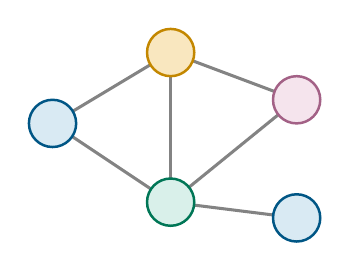
\begin{tikzpicture}[line width=0.9pt]
  \coordinate (a) at (0,1.2); \coordinate (b) at (1.5,2.1); \coordinate (c) at (1.5,0.2); \coordinate (d) at (3.1,1.5); \coordinate (e) at (3.1,0);
  \foreach \p/\q in {a/b,a/c,b/c,b/d,c/d,c/e}{\draw[otgray!75, line width=1.1pt] (\p) -- (\q);}
  \filldraw[draw=otblue!75!black, fill=otblue!15] (a) circle[radius=0.3]; \filldraw[draw=otorange!85!black, fill=otorange!25] (b) circle[radius=0.3]; \filldraw[draw=otteal!75!black, fill=otteal!15] (c) circle[radius=0.3];
  \filldraw[draw=otpurple!80!black, fill=otpurple!20] (d) circle[radius=0.3]; \filldraw[draw=otblue!75!black, fill=otblue!15] (e) circle[radius=0.3];
\end{tikzpicture}
\end{document}
